%% LaTeX Beamer presentation template (requires beamer package)
%% see http://bitbucket.org/rivanvx/beamer/wiki/Home
%% idea contributed by H. Turgut Uyar
%% template based on a template by Till Tantau
%% this template is still evolving - it might differ in future releases!

\documentclass{beamer}

\mode<presentation>
{
\usetheme{Malmoe}

\setbeamercovered{transparent}
}

\usepackage[brazil]{babel}
\usepackage[utf8]{inputenc}
\usepackage[T1]{fontenc}
\selectlanguage{brazil}

\usepackage{graphicx}
\usepackage{subfig}



% font definitions, try \usepackage{ae} instead of the following
% three lines if you don't like this look
\usepackage{mathptmx}
\usepackage[scaled=.90]{helvet}
\usepackage{courier}

\addtobeamertemplate{navigation symbols}{}{
    \usebeamerfont{footline}%
    \usebeamercolor[fg]{footline}%
    \hspace{1em}%
    \insertframenumber/\inserttotalframenumber
}


\setbeamercolor{footline}{fg=blue}
\setbeamerfont{footline}{series=\bfseries}

\title{Apresentação das Atividades de Estágio}

%\subtitle{}

% - Use the \inst{?} command only if the authors have different
%   affiliation.
%\author{F.~Author\inst{1} \and S.~Another\inst{2}}
\author{Gustavo Ciotto Pinton}
\institute{
Grupo de Controle \\
Laboratório Nacional de Luz Síncrotron - LNLS \\ 
Centro Nacional de Pesquisa em Energia e Materias - CNPEM \\ } 

\date{\today}


\usepackage{pgf}
\newcommand{\nologo}{\setbeamertemplate{logo}{}}
\logo{\pgfputat{\pgfxy(0,6.4)}{\pgfbox[right,base]{
\includegraphics[height=1.0cm]{image/CNPEM_LNLS}}}}

\begin{document}

\begin{frame}
\titlepage
\end{frame}

\begin{frame}
\frametitle{Sumário}
\tableofcontents

\end{frame}

\section {Implementação de um servidor NTP}

%\subsection{Introdução}

\begin{frame}
\frametitle{Implementação de um servidor NTP}
\framesubtitle{Introdução}

\begin{itemize}
  \item Problema: rede de controle do \textit{Sirius} será isolada. Como
  sincronizar todos os \textit{logs}?
  \item Receptadores GPS fornecem:
  \begin{itemize}
    \item Horário no formato UTC.
    \item Pulsos 1PPS (\textit{pulse-per-second}), indicando o início de um novo
    segundo e precisão na ordem de nanosegundos.
  \end{itemize}
  \item NTP + Hora UTC + 1PPS = servidor de \textit{stratum 1}
  
  \item 3 modelos comprados:
  \begin{itemize}
    \item \textit{Ultimate GPS Breakout} da \textit{Adafruit}.
    \item \textit{GPS Click} da \textit{MikroElektronika}. 
    \item \textit{CAM M8Q} da \textit{ublox}.
  \end{itemize} 
\end{itemize}

\end{frame}

\begin{frame}
\frametitle{Implementação de um servidor NTP}
\framesubtitle{Instalação}


\begin{itemize}
  \item \textit{Ultimate GPS Breakout}:
  \begin{figure}[h]
    \centering
    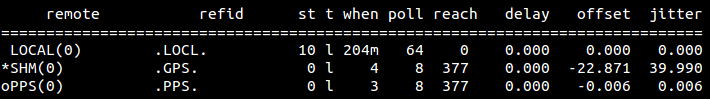
\includegraphics[width=0.80\textwidth]{image/adafruit_GPS}
    \label{img:adafruit} 
  \end{figure} 
  \item \textit{GPS Click}:
  \begin{figure}[h]
    \centering
    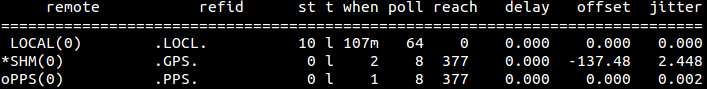
\includegraphics[width=0.80\textwidth]{image/mikroe}
    \label{img:mikroe} 
  \end{figure} 
  \item Comparação:
  \begin{figure}[h!]
    \centering
    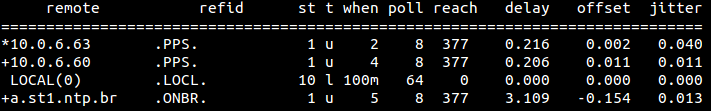
\includegraphics[width=0.80\textwidth]{image/cliente-ntp}
    \label{img:cliente_ntp} 
\end{figure} 
\end{itemize}

\end{frame}

%\subsection{Implementação de variáveis EPICS}
 
\begin{frame}
\frametitle{Implementação de um servidor NTP}
\framesubtitle{Variáves EPICS - \textit{daemon NTPD}}

\begin{itemize}
  \item Variáveis EPICS definidas para o \textit{daemon NTPD} :
  
  \vspace{12pt}
  
	\begin{itemize}
	\item  \textcolor{red}{\textbf{\texttt{NTP:Leap}}: indicação de um eventual
	\textit{leap second} pendente.}
	\item \texttt{NTP:Stratum}: \textit{stratum} do servidor.
	\item \texttt{NTP:Refid}: ID de referência da fonte de sincronismo.
	\item \textcolor{red}{\textbf{\texttt{NTP:Offset}}: \textit{offset} entre o
	relógio do sistema e da fonte.}
	\item \textcolor{red}{\textbf{\texttt{NTP:Jitter}}: desvio padrão das medidas
	\textit{offset} mais recentes.}
	\item \texttt{NTP:Precision}: precisão do \textit{clock} do sistema em \textit{log2}.
	\item \texttt{NTP:Srcadr}: endereço IP do servidor. 			
	\item \texttt{NTP:Version}: versão e data de compilação.
	\item \textcolor{red}{\textbf{\texttt{NTP:Timestamp}}: diferença, em segundos,
	entre a data atual do servidor e a \textit{unix epoch} (1 de Janeiro de 1970).}
	\end{itemize}	    
\end{itemize}	

\end{frame}

\begin{frame}
\frametitle{Implementação de um servidor NTP}
\framesubtitle{Variáves EPICS - \textit{daemon GPSD}}

\begin{itemize}
  \item Variáveis EPICS definidas para o \textit{daemon GPSD} :
  \vspace{12pt}
	\begin{itemize}
	\item \textcolor{red}{\textbf{\texttt{GPS:Fix}}: indicação do tipo de
	\textit{fix} (\textit{no fix}, 2D ou 3D \textit{fix}).}
	\item \texttt{GPS:Latitude}: latitude medida pelo GPS.
	\item \texttt{GPS:Longitude}: longitude medida pelo GPS.
	\item \texttt{GPS:Altitude}: altitude medida pelo GPS.
	\item \textcolor{red}{\textbf{\texttt{GPS:Sattelites}}: \textit{string}
	contendo a identificação dos satélites usados para o \textit{fix}.}
	\item \textcolor{red}{\textbf{\texttt{GPS:Timestamp}}: \textit{timestamp}
	fornecido, análogo à mesma variável do servidor NTP.}
	\end{itemize}	    
\end{itemize}
\end{frame}

\begin{frame}
\frametitle{Implementação de um servidor NTP}
\framesubtitle{Interface gráfica} 
\begin{figure}[h]
    \centering
    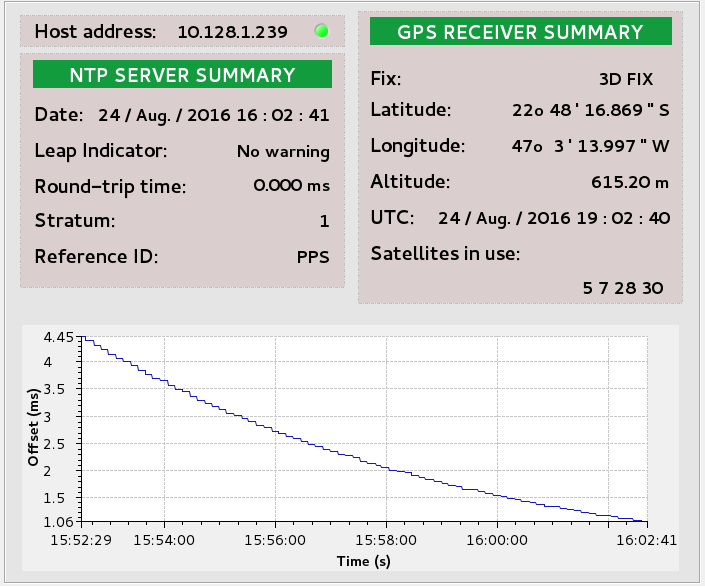
\includegraphics[scale=0.26]{image/epics-opi-ntpgps}
    \caption {Interface construída para visualização das
    \textit{PVs}.}
    \label{img:ntp-opi} 
\end{figure} 

\end{frame}

\section {Sincronização via Ethernet com a BeagleBone Black}

\begin{frame}
\frametitle{Sincronização via Ethernet com a BBB }
\framesubtitle{Introdução}
\begin{itemize}
  \item Objetivo: avaliar o envio de \textit{triggers} de sincronismo via
  \textit{Ethernet}.
  \begin{itemize}
    \item Quantificar o \textit{jitter}, já que o \textit{delay} pode ser
    corrigido.
  \end{itemize}
  \item Propósito geral:
  \begin{itemize}
  \item \textit{BB1}: prepapar os
  pacotes \textit{UDP} contendo \textit{triggers} e enviá-los.
  
  \item \textit{BB2}: espera pacotes \textit{UDP}. Quando recebe, atualiza seu
  contador e seus pinos de saída.
  \end{itemize}
  \item 2 implementações realizadas: 
  \begin{itemize}
    \item \textit{Linux Kernel Modules}.
    \item PRU - \textit{Programmable Real-time Unit}.
  \end{itemize}
\end{itemize}
\end{frame}

\begin{frame}
\frametitle{Sincronização via Ethernet com a BBB }
\framesubtitle{Introdução}
\begin{itemize}
  \item Implementação dos \textit{Kernel Modules}:
\end{itemize}

\vspace{-12pt}

\begin{columns}

\begin{column}{.33\textwidth}

\begin{figure}[h!]
	
  \centering
  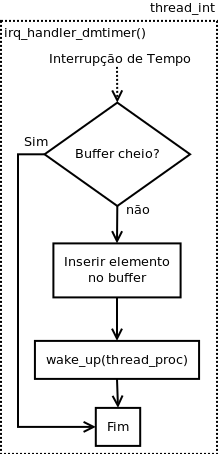
\includegraphics[scale=0.260]{image/thread_int}
  \caption{\centering BB1: \textit{thread} que é interrompida pelo
  \textit{timer}.}
  \label{fig:thread_int}
\end{figure}
\end{column}
		  
\begin{column}{.33\textwidth}

\begin{figure}[h!]
		  \centering
		  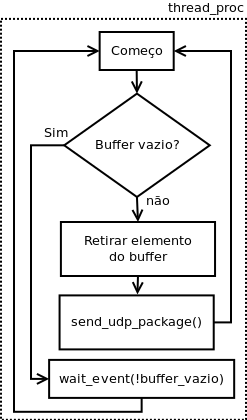
\includegraphics[scale=0.260]{image/thread_proc}
		  \caption{\centering BB1: \textit{thread} que envia pacotes à
		  rede.}
		  \label{fig:thread_proc} 
\end{figure}
\end{column}

\begin{column}{.33\textwidth}

\begin{figure}[h!]
			\centering
			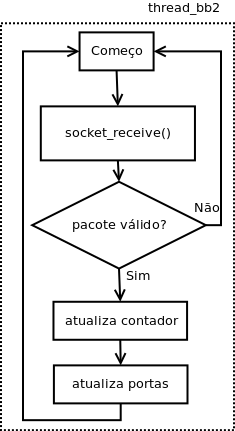
\includegraphics[scale=0.260]{image/thread_bb2}
			\caption {\centering \textit{thread} do \textit{kernel module}
			em
			\texttt{BB2}.}
			\label{fig:thread_bb2}
\end{figure}
\end{column}

\end{columns}
\end{frame}

\begin{frame}
\frametitle{Sincronização via Ethernet com a BBB }
\framesubtitle{Resultados}

\vspace{-24pt}

\begin{columns}

\begin{column}{.5\textwidth}

\begin{figure}[h!]
\centering
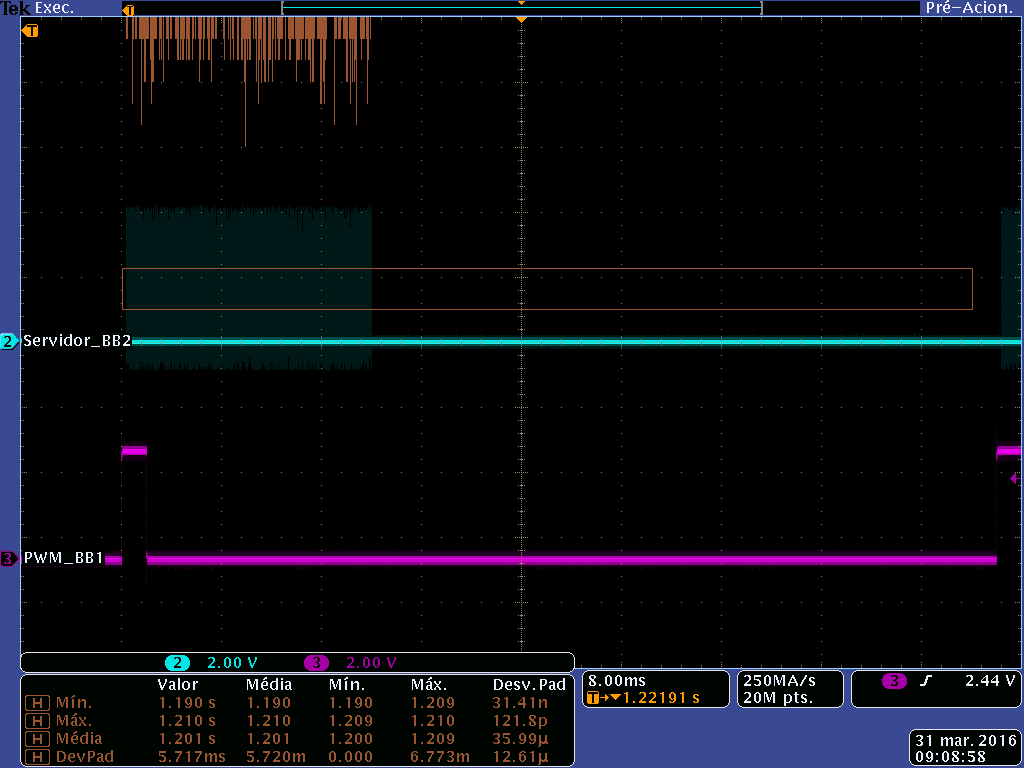
\includegraphics[scale=0.16]{image/tek_com_threads}
\caption {\centering Captura de tela do osciloscópio para a implementação com
\textit{kernel modules}.}
\label{fig:osciloscopio_thread}
\end{figure}
\end{column}
		  
\begin{column}{.5\textwidth}

\begin{figure}[h!]
\centering
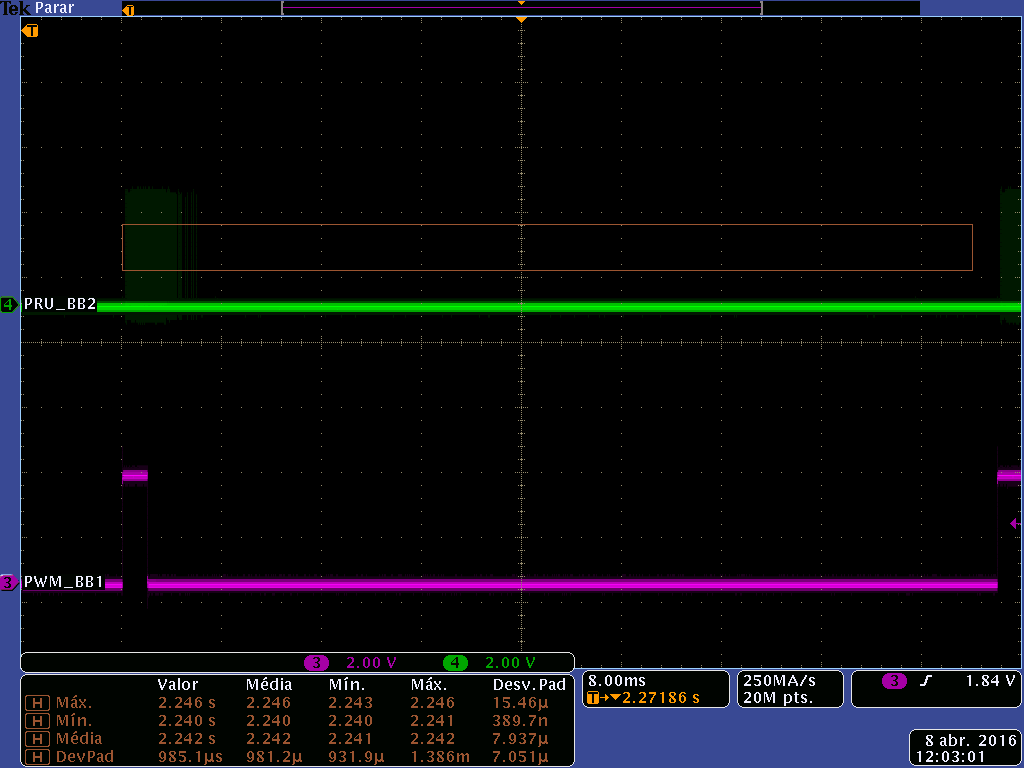
\includegraphics[scale=0.16]{image/tek_pru}
\caption {\centering Captura de tela do osciloscópio para implementação com
PRU.}
\label{fig:pru_osciloscopio_thread}
\end{figure}
\end{column}

\end{columns}
\end{frame}

\section {Manutenção do PROSAC e Implementação de Aplicações Clientes}
%\subsection{Introdução}

\begin{frame}
\frametitle {\textit{Firmware} de controle PROSAC}
\framesubtitle{Introdução}

\begin{itemize}
  \item Firmware desenvolvido no grupo de controle.
  \item Propósito é receber requisões da sala de controle e acionar a respectiva placa do bastidor. 
  \item Suporta diversas placas que são usadas atualmente no UVX:
  \begin{itemize}
    \item LOCON de 12 e 16 bits.
    \item STATFNT.
    \item DIGINT.
    \item \ldots
   \end{itemize}
   \item Atualmente, executadas sobre o \textit{single-board computer Advantech
   PCM-4153F}:
   \begin{itemize} 
   		\item Problema: alto custo das SBCs.
   \end{itemize} 
\end{itemize}

\end{frame}

%\subsection{Manutenção do PROSAC}

\begin{frame}
\frametitle {Manutenção do PROSAC}

\begin{itemize}
  \item Migração para a \textit{BeagleBone}: solução mais barata e forte
  comunidade.
  \item Artigo na PCaPAC 2016: \textcolor{red}{\textit{UVX Control System: An
  Approach With BeagleBone Black}}.
  \item Tarefa: ajustar a política de escalonamento e a prioridade das
  \textit{threads}, de forma a obter o melhor desempenho possível nas tarefas
  síncronas (uso do \textit{Completely Fair Scheduler}).
\end{itemize}

\vspace{-12pt}
\begin{table}[h]

	\centering
	\caption{\label{tab:prosac} Resultados do \textit{PROSAC} com o
	\textit{Completely Fair Scheduler}.}
	\begin{tabular}{| c | c | c | c |}
		\hline
		\textbf{Frequência (Hz)} & \textbf{Pulsos perdidos} & \textbf{Total} &
		\textbf{Razão} \\ \hline 
		150 & 0 & 579.812  & 0 \\ \hline
		512 & 8 & 5.376.056 & 0.0001\% \\ \hline
		1000 & 18 & 6.050.225 & 0.0003\% \\ \hline
	\end{tabular}	    
\end{table}

\end{frame}

%\subsection{Implementação de Clientes do PROSAC}

\begin{frame}
\frametitle {Implementação de Clientes do PROSAC}

\begin{itemize}
  \item Cliente em JAVA:	 
\end{itemize}

\begin{figure}
\centering
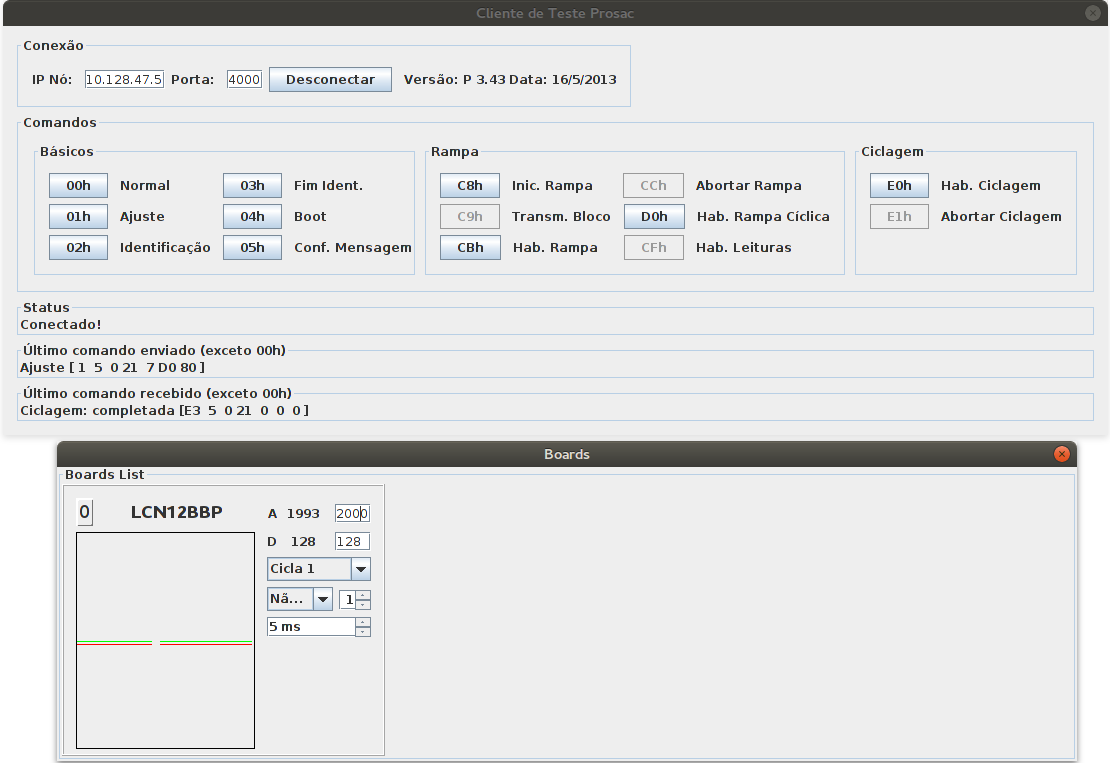
\includegraphics[width=0.7\textwidth]{image/prosac-java}
\caption {Cliente PROSAC baseado em JAVA.}
\label{fig:login}
\end{figure}
 
\end{frame}

\begin{frame}
\frametitle {Implementação de Clientes do PROSAC}

\begin{itemize}
  \item Cliente baseado no \textit{kit} \textit{STM32F7 Discovery}:	
  
  \begin{itemize} 
  \item Configuração da interface \textit{OpenOCD}.
  \item \textit{STMCubeMX} para inicialização dos pinos.
  \item Adição dos \textit{middlewares} \textit{FreeRTOS} e \textit{LwIP} ao
  projeto.
  \item Correção do \path{stm32f7_hal_conf.h} com a definição dos
  registradores corretos do módulo \textit{PHY}.
  \end{itemize}
\end{itemize}

\vspace{-12pt}

\frametitle {Implementação de Clientes do PROSAC}
\begin{figure}[h]
\centering
\subfloat[Tela inicial. \label{fig:1}]{
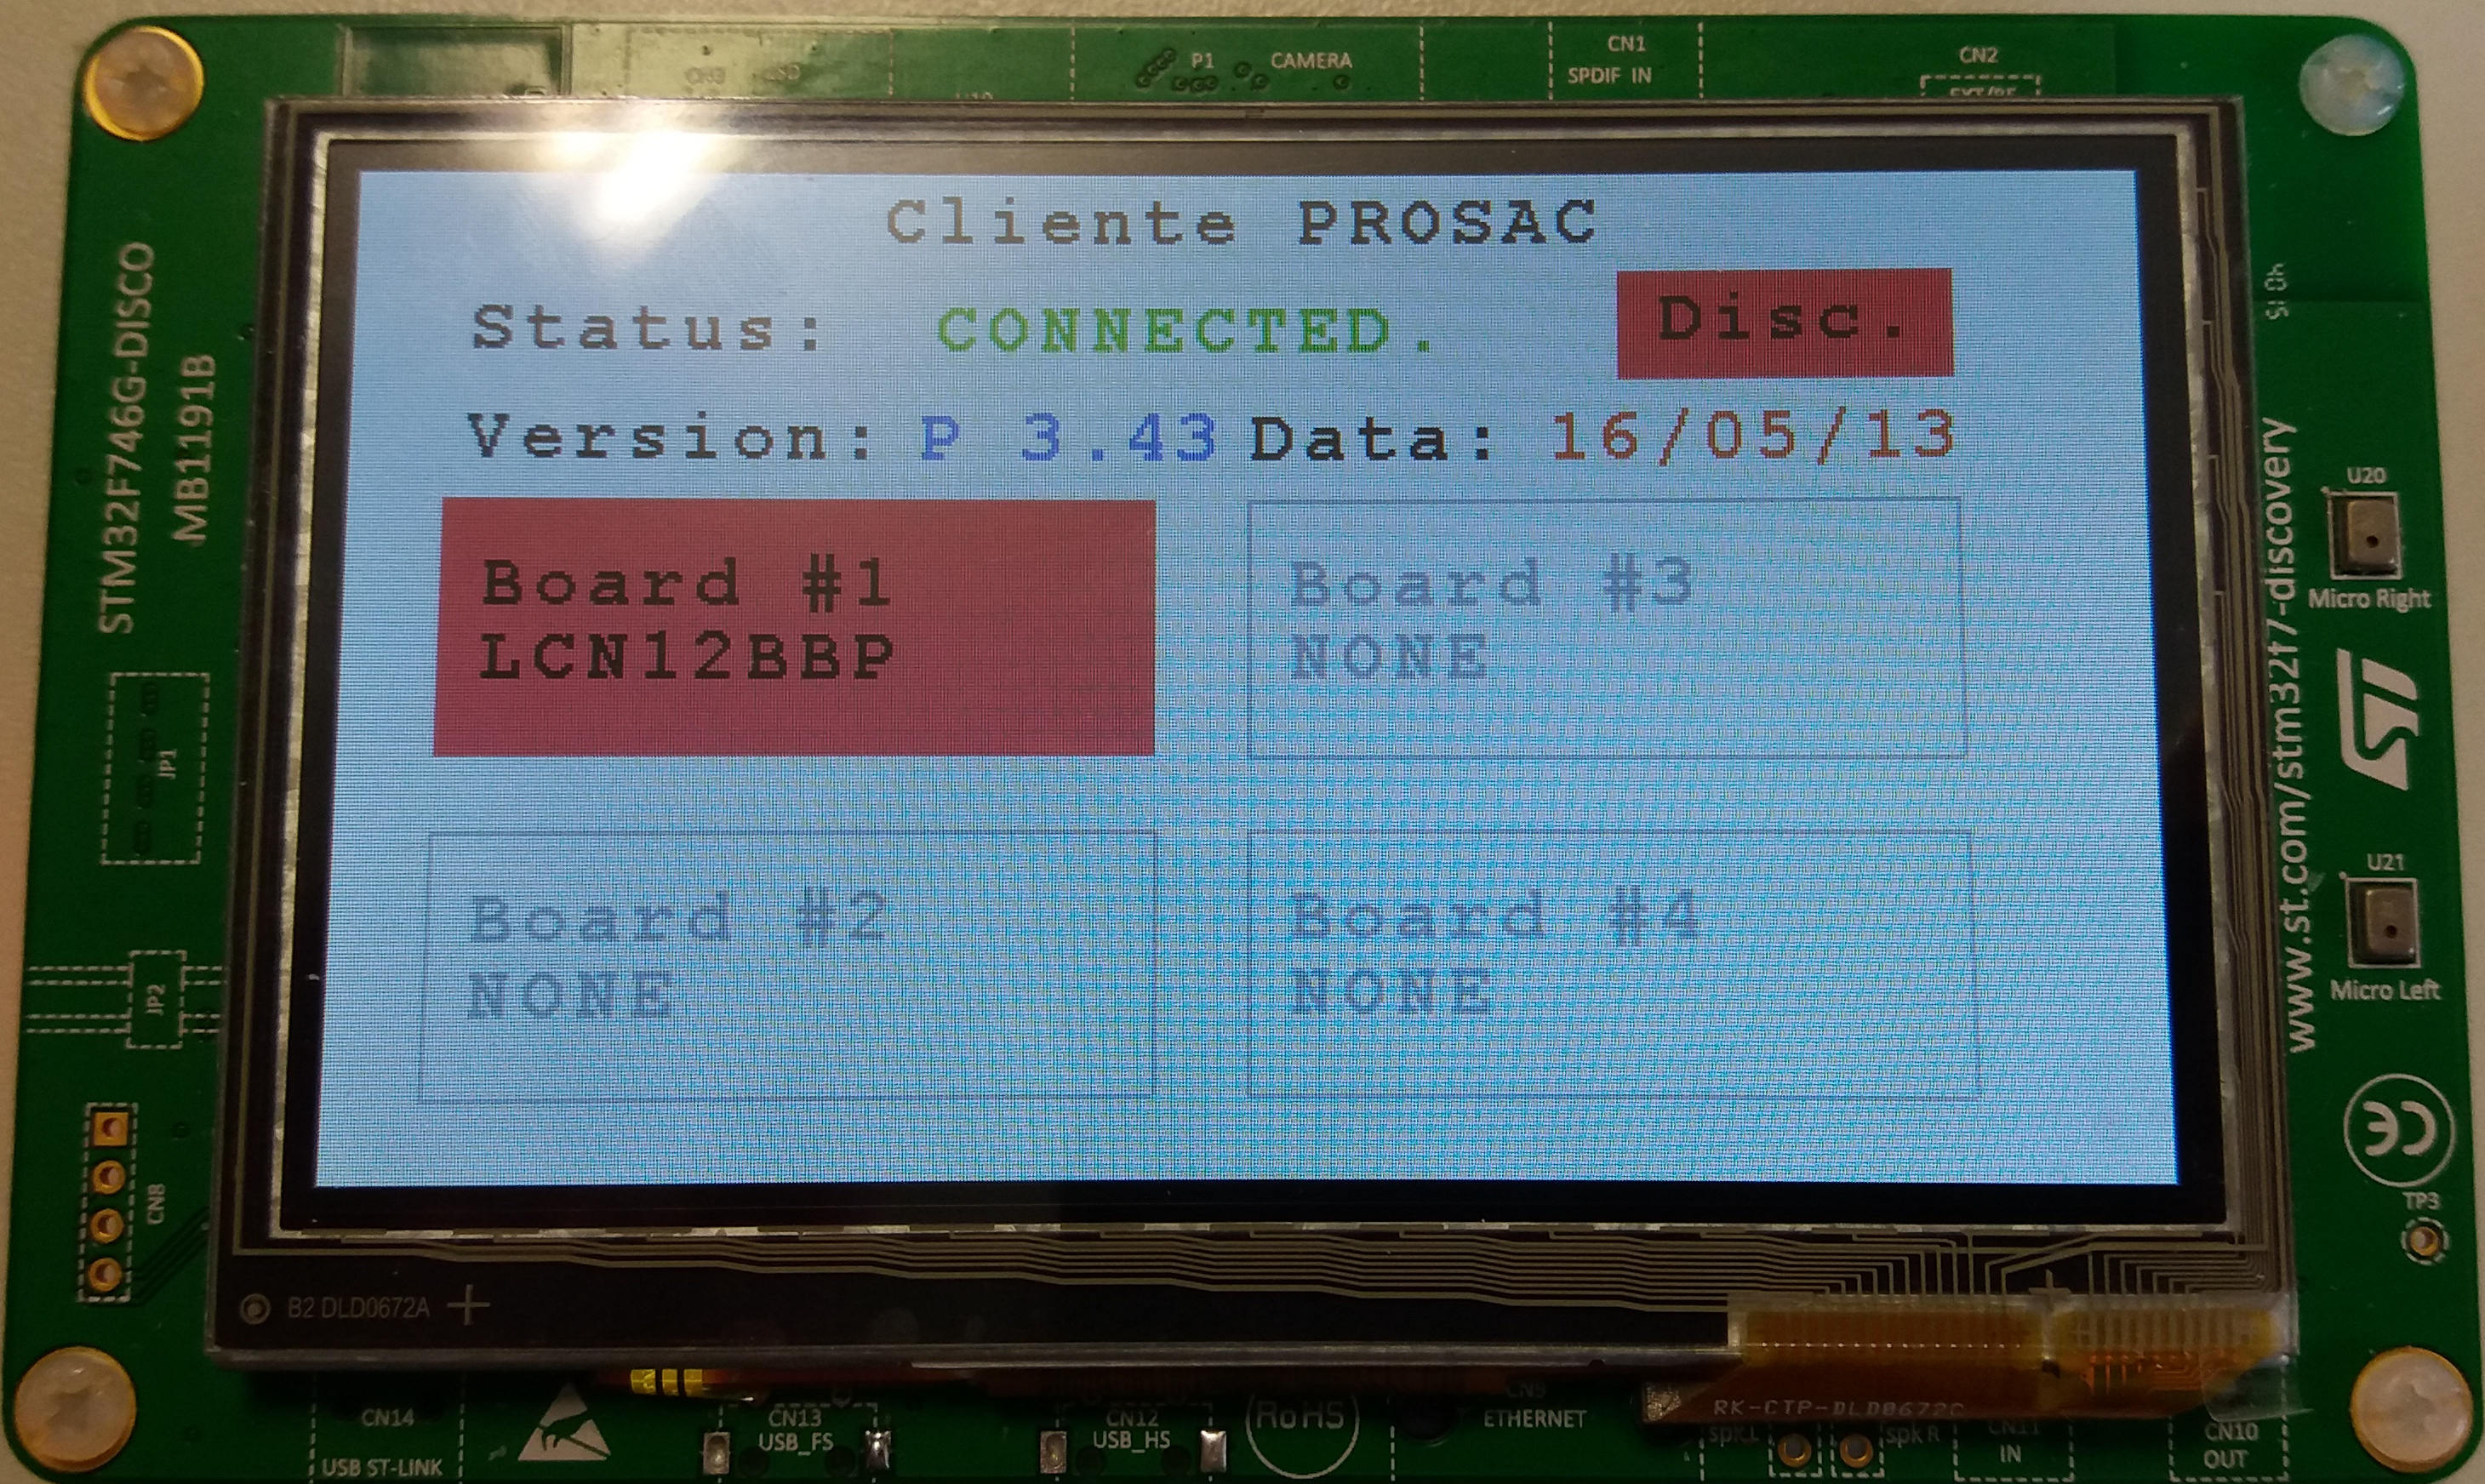
\includegraphics[width=4.65cm]{image/stm32}}
%
\subfloat[Tela de comandos de cada placa. \label{fig:2}]{
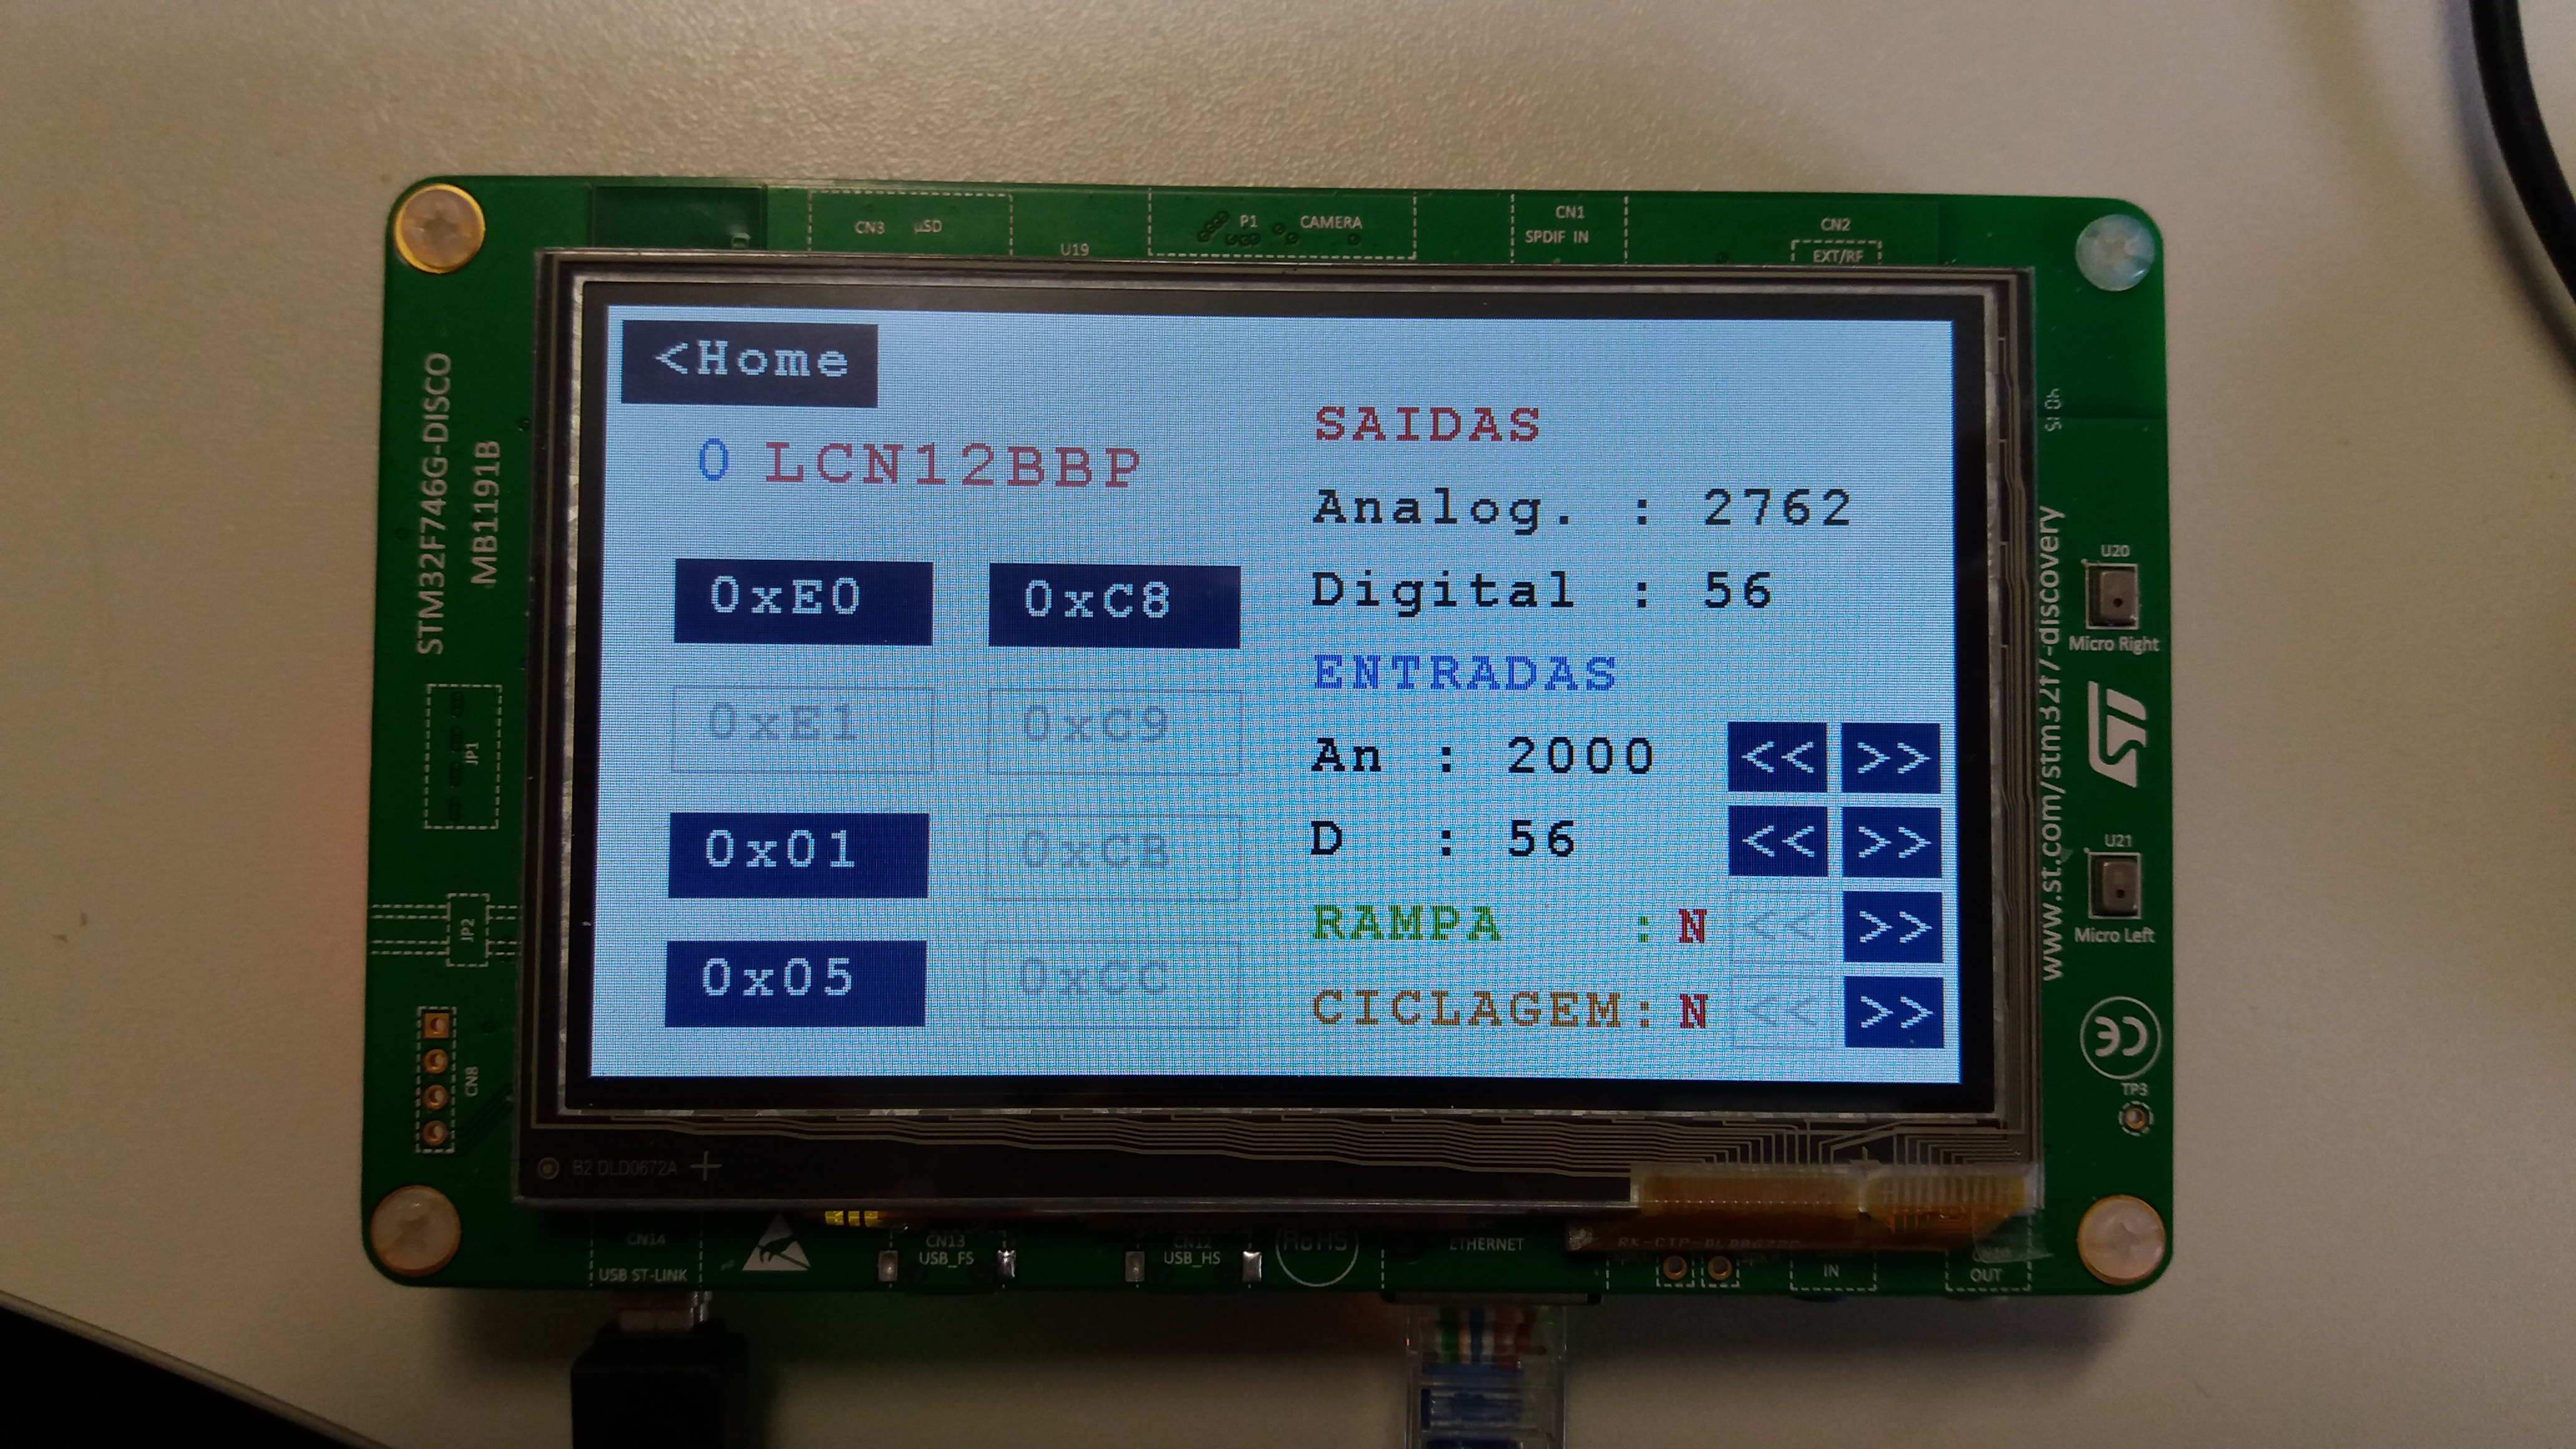
\includegraphics[width=4.65cm]{image/stm32-2}}
\vspace{-12pt}
\caption {Cliente PROSAC baseado no \textit{kit} \textit{STM32F7 Discovery}.}
\label{fig:stm32}
\end{figure}

\end{frame}

\section {Arquivador de variáveis EPICS}
%\subsection{Introdução}

\begin{frame}
\frametitle {Arquivador de variáveis EPICS}
\framesubtitle{Introdução} 

\begin{itemize}
  \item \textit{Management}: gerência da \textit{appliance}.
  \item \textit{Engine}: integração entre os módulos.
  \item \textit{Data Retrieval}: recuperar os dados das \textit{PVs} arquivadas.
  \item \textit{ETL}: extrair os dados das unidades de armazenamento.

\end{itemize}

\begin{figure}[h]

    \centering
    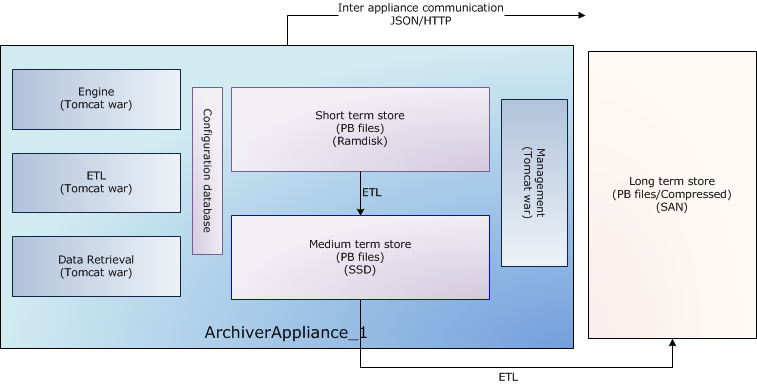
\includegraphics[scale=0.3]{image/applarch}
    \caption {Modo de funcionamento de uma \textit{appliance}.}
    \label{fig:epics_archiver}
\end{figure}

\end{frame}

%\subsection{Modificações}

\begin{frame}
\frametitle {Arquivador de variáveis EPICS}
\framesubtitle{Modificações}

\begin{itemize}
  \item Interfaces de \textit{login}:
  \begin{itemize}
    \item Problema: qualquer pessoa logada pode inserir ou remover variáveis do
    sistema.
    \item Instalação de um servidor LDAP: no futuro, integrar com o servidor
    LDAP do CNPEM.
    \item Módulo PHP: realiza a comunicação entre servidor LDAP e usuário e
    retorna se a autenticação foi bem sucedida ou não.
    \item Em caso de sucesso, outra requisição POST é enviada ao módulo de
    \textit{management}.
    \item Módulo de \textit{management}: inicia uma nova sessão para o usuário.
  \end{itemize}
  \item Modificações nos arquivos \texttt{.css}.
\end{itemize}

\end{frame}

%\subsection{Resultados}

\begin{frame}
\frametitle {Arquivador de variáveis EPICS}
\framesubtitle{Resultados}

\begin{figure}[h]

\centering
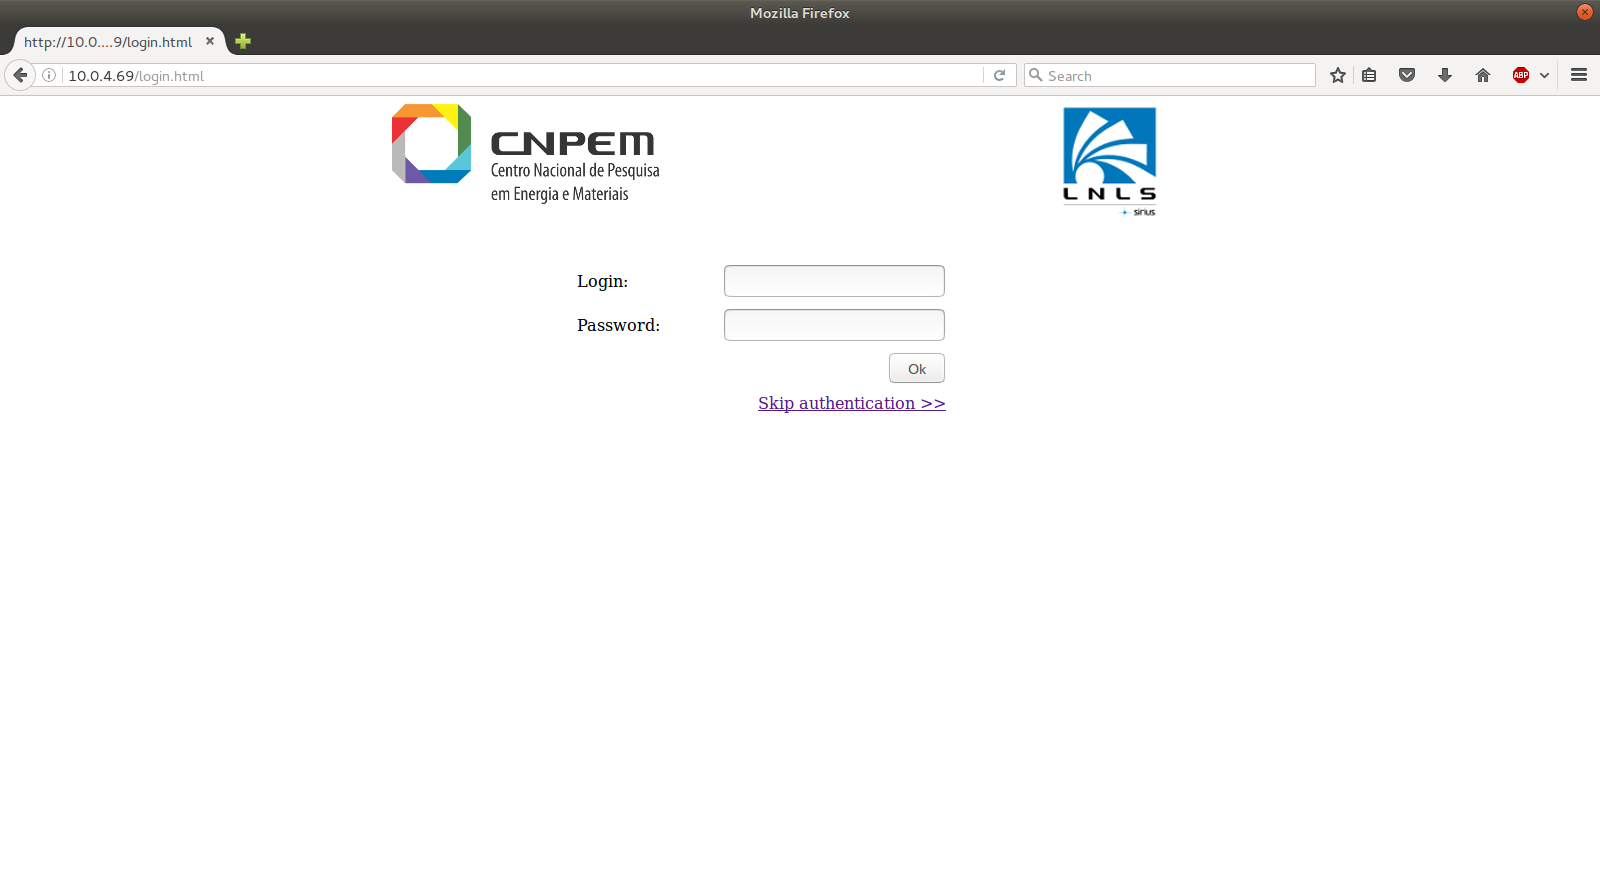
\includegraphics[width=0.93\textwidth]{image/login}
\caption {tela de \textit{login} para o \textit{archiver} instalado no OPR23.}
\label{fig:login}
\end{figure}

\end{frame}

\begin{frame}
\frametitle {Arquivador de variáveis EPICS}
\framesubtitle{Resultados}

\begin{figure}[h]

\centering
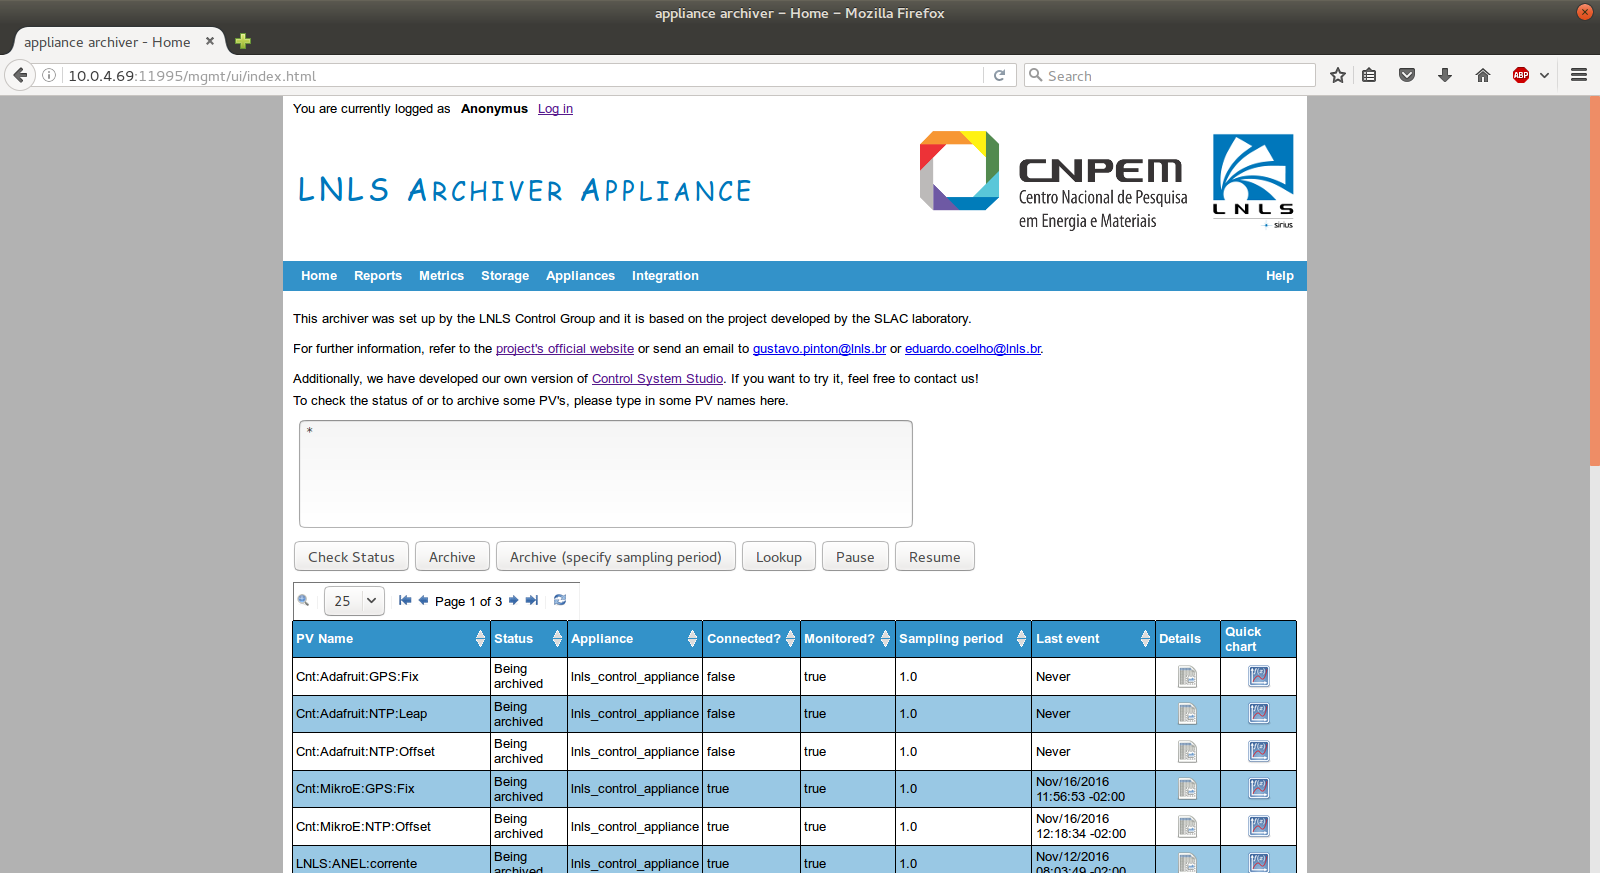
\includegraphics[width=0.93\textwidth]{image/archiver}
\caption {\textit{Archiver} instalado no OPR23.}
\label{fig:archiver}
\end{figure}

\end{frame}

\section {Servidor de alarmes BEAST}
%\subsection{Introdução}

\begin{frame}
\frametitle{Servidor de alarmes BEAST}
\framesubtitle{Introdução}
\begin{itemize}
  \item Capaz de gerenciar e controlar os alarmes gerados pelos servidores
  EPICS disponíveis na rede.
  \item Implementado em \textit{Java} e baseado no \textit{Eclipse}.
\end{itemize}

\begin{figure}[h]

\centering
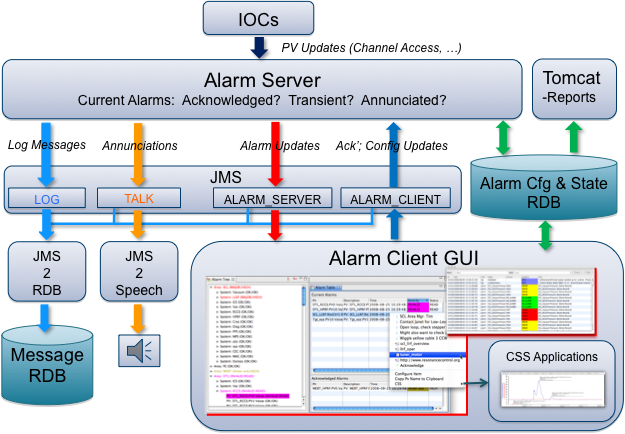
\includegraphics[scale=0.25]{image/beast-arquitetura}
\caption {Implementação do sistema de monitoramento de alarmes
\textit{BEAST}.}
\label{fig:best_arquitetura}
\end{figure}

\end{frame}

%\subsection{Instalação}

\begin{frame}
\frametitle{Servidor de alarmes BEAST}
\framesubtitle{Cliente do Servidor de Alarmes - CSStudio}
\begin{figure}[h]
\centering
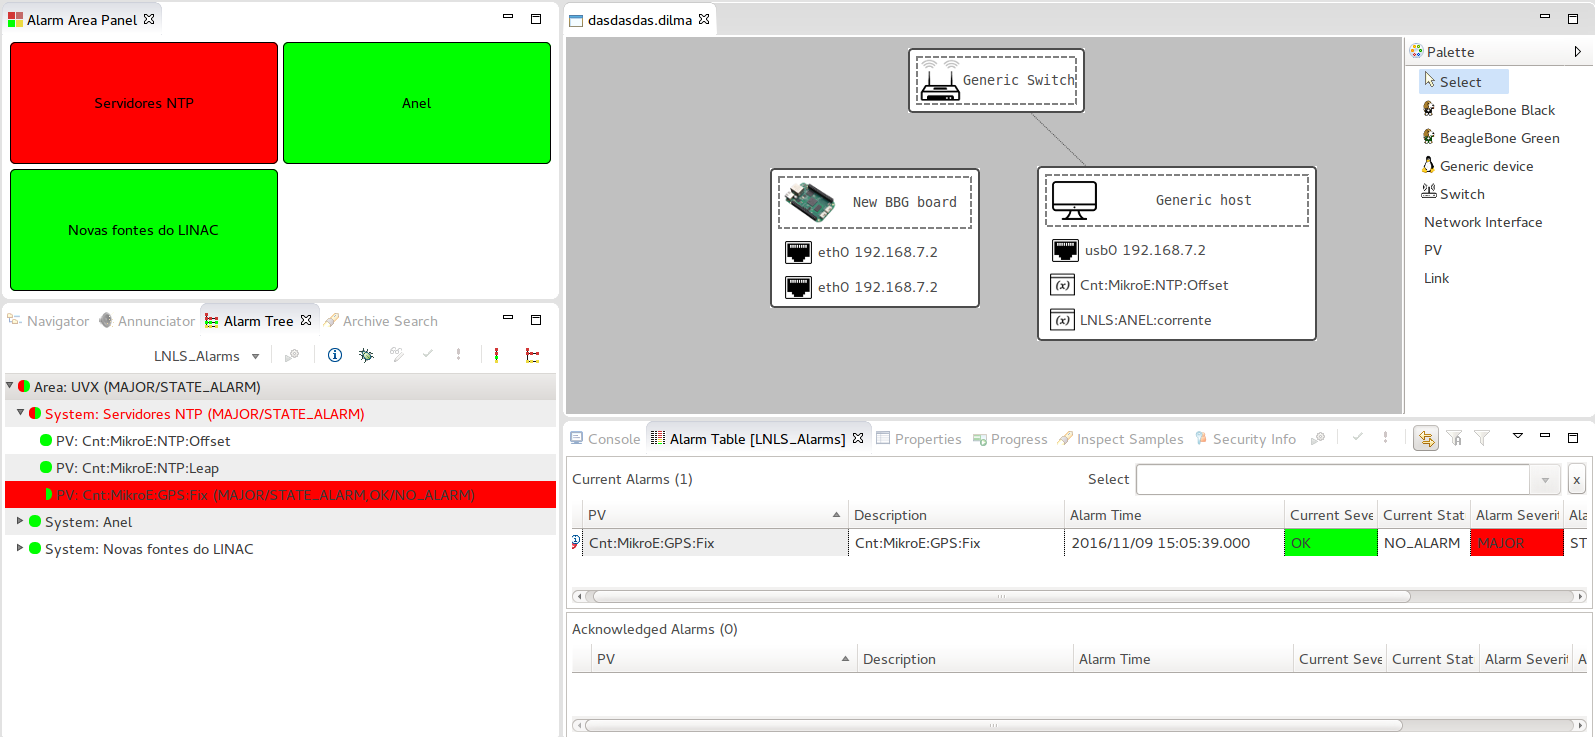
\includegraphics[width=\textwidth]{image/beast-screen-shot}
\caption {Cliente \textit{BEAST} baseado no \textit{Control System Studio}.}
\label{fig:alarm}
\end{figure}

\end{frame}

%\subsection{Obtendo o LNLStudio}

\begin{frame}
\frametitle{Servidor de alarmes BEAST}
\framesubtitle{Obtendo o LNLStudio - CSStudio 4.3 e Luna}
\begin{figure}[h]
\centering
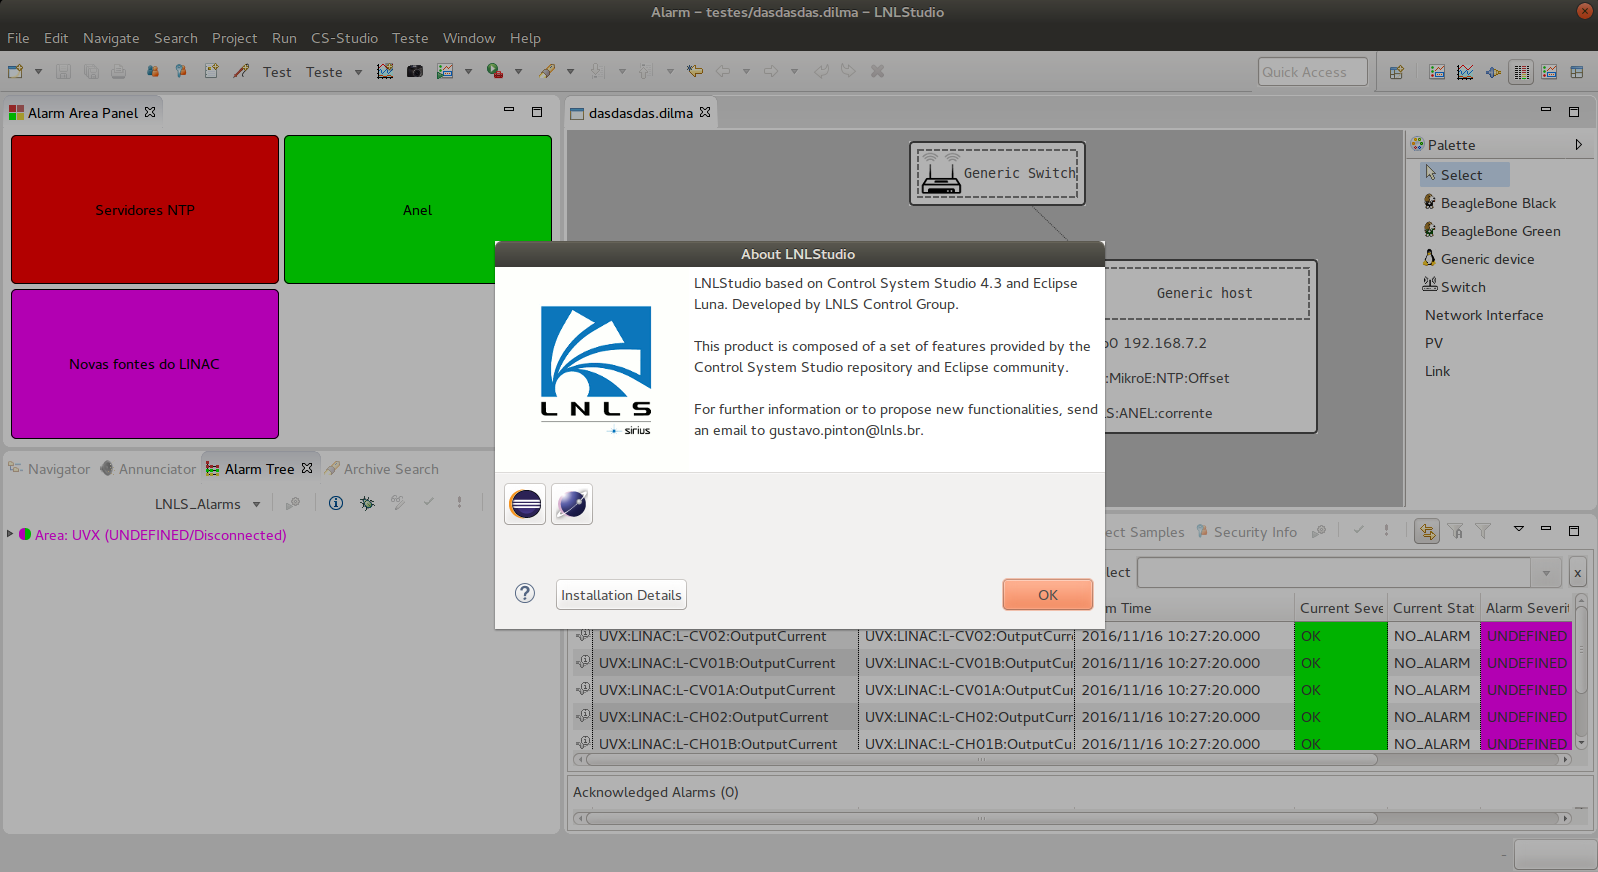
\includegraphics[width=0.90\textwidth]{image/lnlstudio}
\caption {\centering Produto \textit{LNLStudio} exportado a partir de uma
configuração do \textit{Eclipse}.}
\label{fig:lnlstudio}
\end{figure}

\end{frame}

\begin{frame}
\frametitle{Referências}

{\small
\begin{itemize}
  \item Linuxpps installation. 
  \url{http://linuxpps.org/wiki/index.php/LinuxPPS_installation}. Acessado em 08 de Novembro de 2016.
  \item Mills D and Martin J. Network time protocol version 4: protocol and
  algorithm specification. Request for Comments RFC 5905, Junho 2010.
\item  Kay Kasemir, Xihui Chen, and Katia Danilova. Best ever alarm system
toolkit. \url{http://www.aps.anl.gov/epics/meetings/2010-10/14/BEAST_EpicsMeeting2010.pdf} . Acessado em 11 de Setembro de 2016.
\item S. Lescano, A. R. D. Rodrigues, E. P. Coelho, G. C. Pinton, J. G. R. S.
 Franco, and P. H. Nallin. Uvx control system: An approach with beaglebone
 black. Personal Computers and Particle Accelerator Controls, 2016.
\end{itemize}
}
\end{frame}

\begin{frame}
\frametitle{Referências}
{\small
\begin{itemize}
\item Robert Love. Linux Kernel Development. Pearson Education, Inc., 3rd
edition, 2010.
\item Gary E. Miller and Eric S. Raymond.
Gpsd time service
howto.\url{http://www.catb.org/gpsd/gpsd-time-service-howto.html}. Acessado em 08 de Novembro de 2016.
\item Derek Molloy. Writing a linux kernel module — part 1: Introduction.
\url{http://derekmolloy.ie/ writing-a-linux-kernel-module-part-1-introduction/}. 
Acessado em 12 de Abril de 2016.
\end{itemize}
}

\end{frame}


\end{document}
